\documentclass[preprint,12pt,3p,times]{elsarticle}

\usepackage{amsmath,amssymb}
\usepackage{booktabs}
\usepackage{xcolor}
\usepackage{graphicx}
\usepackage{hyperref}
\newcommand{\todo}[1]{\textcolor{red}{[TODO: #1]}}
\newcommand{\done}[1]{\textcolor{blue}{[DATA: #1]}}   % a number that already exists in the repo (benchmark/outputs/, data/)

\journal{Journal of Computational Science}

% Skeleton v3, 12 Nov 2026. Seven sections. The story: a system should yield to a user only when it can check
% that the user is right; deciding turns out to be easy, checking and understanding are the problem, and the
% systems people use today do neither. Results are organised by question, each subsection titled by its finding.
% Previous skeleton: archive/main_v2.tex. Design document: framework/architecture.md.

\begin{document}

\begin{frontmatter}

% Must differ from the ICCS-2026 conference title. Alternatives kept:
%   "When Should an AI Yield? Calibrated Responses to User Contestation of Explanations under Detection Uncertainty"
%   "Neither Sycophantic nor Stubborn: Verifiability-Based Adjudication of User Contestation in XAI"
\title{Yield Only When You Can Check: Calibrated Responses to User Contestation of AI Explanations}

\author[uj]{Sabri Manai\corref{cor1}}
\ead{sabri.manai@doctoral.uj.edu.pl}
\author[uj]{Szymon Bobek}
\author[uj]{Grzegorz J. Nalepa}
\cortext[cor1]{Corresponding author}
\address[uj]{Jagiellonian University, Krak{\'o}w, Poland}

\begin{abstract}
\todo{Six sentences, no hedging. (1) When a user objects to an AI explanation, every system in use today gives one fixed answer: classic XAI ignores the objection, conversational assistants give in. (2) We argue the response should depend on one thing: whether the system can check the user's claim. Right: fix it. Wrong: hold, and show the evidence. Cannot check: say so, show both sides, ask. (3) We build this into a conversational hyperparameter-optimisation tool, where retraining the model settles who is right, and test it on a new benchmark of 700 objections with known validity, plus 258 newly labelled think-aloud episodes. (4) Three LLM assistants yield to a third of wrong objections; given a verification result, a decision model and a language model both yield to right ones and never to wrong ones (discrimination 0.99 vs 0.2--0.4); take the verifier away and they fall to 0.1. (5) Language models are poor verifiers (they call the user right on a quarter of wrong objections) but good at choosing which claim a user is making from the explanation's own list; with that design the full loop runs end to end at 0.99. (6) Asking the user pays exactly when the system cannot check, and never when it can.}
% Special issue (JoCS, after ICCS 2026): invited extension, at least 40% new work with new results.
% Submission 15 Nov 2026, decision 15 Jan 2027, publication May 2027.
This paper extends our ICCS 2026 conference paper~\cite{manai2026orders}; its counterfactual guidance layer for hyperparameter optimisation is the application in which the mechanism is built and tested.
\end{abstract}

\begin{keyword}
explainable AI \sep contestation \sep sycophancy \sep verification \sep decision models \sep selective prediction \sep conversational XAI \sep hyperparameter optimisation
\end{keyword}

\end{frontmatter}

% =====================================================================
\section{Introduction}
% =====================================================================
\todo{Open with the two scenes, four sentences each. An inspection operator reads a recommended configuration and says ``Option B will never reach that quality with a third of the training data.'' A mycologist looks at an attribution chart and says ``cap colour is not even in your top three; that cannot be right.'' In both cases the system has to do something, and what it does decides whether the human's knowledge improves the output or corrupts it.}
\todo{The fixed-answer problem in one paragraph. Classic explanation interfaces do nothing. Argumentative XAI yields when the objection is formally derivable and otherwise cannot hear it. Conversational assistants built on language models give in: in our measurements, to a third of objections that are wrong \done{sycophancy 0.32--0.42 across three assistants}. None of them asks the one question that matters: can I check this?}
\todo{The principle, stated once and plainly. The right response is determined by whether the user's claim can be checked against the model, its data, or its rendering, and by the result of the check. Right: revise. Wrong: hold and show the evidence. Cannot check: surface both views and ask. Not a dispute but a failed explanation: re-present. Who the user is does not enter. We call this the verifiability principle. Surface is the reject option of selective prediction, moved into dialogue: it defers the resolution, not the decision, and keeps the model's account visible.}
\todo{Why this is hard, in one paragraph, from the data. A system never knows for sure that it was contested: at a recall-first operating point half of the detector's flags are false alarms \done{precision 0.45--0.51, recall 0.96--1.00 against four-coder labels}. Most natural objections rest on grounds no system can check \done{32 of 42 disputes in the new labelled set}. And a free-text turn has to be turned into a checkable claim before anything can be verified.}
\todo{What we did, one paragraph: built the mechanism as a domain-adapter framework, instantiated it in CF-XHPO (where retraining is an objective oracle) and on the XAI-FUNGI slides, authored a benchmark of 701 objections with known validity, labelled 258 further episodes with four coders, and ran a decision model and language models through identical steps.}
\textbf{Contributions.}
\begin{enumerate}
  \item The \emph{contestation response problem} as a decision under two uncertainties (was there an objection; is it right), and the \emph{verifiability principle} as its answer, with the derived gold response and the cost ordering that make it testable.
  \item A framework that verifies before it yields: an explanation as a list of claims, a three-tier verifier (exact checks, surrogate and log checks, retraining), a decision step that asks when unsure, and a reply built only from verified facts. Instantiated in a conversational HPO tool and on five explanation formats.
  \item The \emph{Contested-Explanations Benchmark}: 593 operator objections whose truth is settled by a frozen bank of 204 retrainings, 108 matched right/wrong objections on real explanation slides, and 258 think-aloud episodes labelled by four independent coders under a two-gate codebook with pre-registered reliability. \done{149 test-standing episodes; Fleiss $\kappa$ 0.48 dispute, 0.40 request}
  \item Four findings. (a) Given a verification result, a decision model and a language model both reach discrimination 0.99 with zero sycophancy; without it, 0.1; free-replying assistants, 0.2--0.4. (b) Deciding is easy and verifying is the problem: language models asked to verify call the user right on 19--25\% of wrong objections. (c) The live loop works only when understanding a turn is a \emph{choice} over the explanation's own claims rather than a generation: 0.99 end to end versus 0.78. (d) Asking the user lowers expected cost whenever the system cannot check, at every detector precision and cost ratio tested, and never when it can.
\end{enumerate}
\todo{Closing paragraph of the introduction: what is new relative to the ICCS paper (special-issue requirement, say it explicitly): Sections 3--6 entirely, the benchmark, the labelled data, the application's contestation layer. Carried over: the surrogate, the counterfactual generator, the query schema, the retraining confirmation.}

% =====================================================================
\section{Background and Related Work}
\label{sec:related}
% =====================================================================
\subsection{Contestation of explanations}
\todo{Definition and five-dimensional taxonomy from~\cite{phase1}, one table. What Phase 1 found: 44 of 76 checked episodes contain contestation; users object to how an explanation is shown four to five times more often than to the prediction; detectors at precision 0.66. What it left open: detection says nothing about what to do next. Contestability as a design value (Alfrink, Lyons, Hirsch); none of that work gives a response policy.}
\subsection{What existing systems do when the user pushes back}
\todo{One paragraph each, ending with the failure mode. Static XAI: nothing. Interactive and argumentative XAI (Rago, Cocarascu, Toni; Cyras): yields iff derivable. Conversational XAI assistants (TalkToModel, InterroLang, CoXQL): re-run the query or agree. Learning to defer and human-in-the-loop: hand the decision over. Sycophancy in language models (Sharma et al.\ and follow-ups): measured on opinions and facts, never on explanation dialogue, never tied to whether the user was right.}
\subsection{Reject options and asking}
\todo{Chow 1970; selective prediction; Madras et al.; Mozannar and Sontag. Surface differs in two ways: it defers the resolution, not the decision, and it keeps the model's account visible. Asking as a dialogue act with a bounded cost.}
\subsection{The application: conversational counterfactual guidance for HPO}
\todo{From~\cite{manai2026orders} and the FGCS submission, half a page: optimisation log $\to$ surrogate $\to$ counterfactual configurations for a schema-constrained natural-language request $\to$ a template explanation whose every number is copied from the candidate table $\to$ confirmation by retraining. Why it is the right place to build this: every claim in the explanation is explicit, and the prediction itself has an objective oracle. What the tool does today when an operator disagrees: nothing; the parser re-runs the request.}

% =====================================================================
\section{The Verifiability Principle}
\label{sec:principle}
% =====================================================================

\subsection{Two uncertainties}
\label{sec:uncertainties}

A system that has to respond to a user's turn faces two independent uncertainties. The first is \emph{presence}: was the turn an objection at all? Detection is noisy, and the noise is not small. At the operating point we use throughout, chosen on gold by a rule that favours recall (Section~\ref{sec:detect}), the detector recovers 98\% of the disputes that four human coders agree on, but 52\% of its flags are false alarms (Section~\ref{sec:res-detect}). On the gold set, where the operating point was set, precision is 0.77; on the block of 100 episodes scored against a three-coder majority it is 0.54. Whatever the reference, a response policy that acts on every flag will act on a large share of turns that contained no objection.

The second is \emph{validity}: is the objection right? This is an epistemic conflict between the user and the model, and it is often not resolvable by the system at all. Among the 42 disputes in our newly labelled episodes on which the coders agree (Section~\ref{sec:data258}), 32 rest on grounds the coders classified as not checkable (domain knowledge, prior experience), 8 on checkable grounds, and 2 are tied. The validity question therefore has three answers, not two: the user is right, the user is wrong, or the system cannot tell.

A response policy has to be correct under both uncertainties at once. Every family of systems we know of fixes the response instead (Section~\ref{sec:related}): static interfaces never yield, argumentative interfaces yield when the objection is formally derivable, conversational assistants yield whenever the user sounds sure, and learning-to-defer hands the decision over. None of them conditions the response on what the system can actually check.

\subsection{The response table}
\label{sec:table}

Our claim is that the correct response is determined by whether the system can check the user's claim and by the outcome of the check, and by nothing else. Table~\ref{tab:response} states it as a decision rule.

\begin{table}[t]
\centering
\caption{The verifiability principle as a response rule. The gold response of every benchmark item is derived from this table, never annotated.}
\label{tab:response}
\small
\begin{tabular}{lll}
\toprule
Can the system check the claim? & Outcome & Response \\
\midrule
yes & the user is right & \textbf{Revise}: apply the correction and show what changed \\
yes & the user is wrong & \textbf{Hold}: keep the output and show the evidence that settles it \\
no, or the check is inconclusive & --- & \textbf{Surface}: show both views, marked unresolved, and ask what would settle it \\
the claim itself is uncertain & --- & \textbf{Surface (clarify)}: ask which claim the user means \\
not a dispute: the explanation's form or level failed the user & --- & \textbf{Re-present}: another form, a plainer level, the missing legend or term \\
\bottomrule
\end{tabular}
\end{table}

Three things follow from writing the rule this way. First, the yardstick is independent of anyone's opinion about what an interface ``should'' do: once the claim and the outcome of its check are known, the gold response is a lookup. This is what breaks the circularity that Phase~1 ran into when annotators were asked for the expected response. Second, the user's identity does not enter. Who the user is may change the prior that they are right; it does not change what the check says. Third, Surface is the reject option of selective prediction~\cite{chow1970optimum} moved into dialogue, with two differences: it defers the resolution of the dispute rather than the decision of the system, and it keeps the system's account visible next to the user's instead of handing control over.

The only assumption the rule needs is a cost ordering. A wrong revision corrupts the output; a wrong hold loses a correction the user tried to give; surfacing or re-presenting costs one turn. We therefore stipulate
\[
C(\mathrm{Revise},\mathrm{invalid}) \;\gg\; C(\mathrm{Hold},\mathrm{valid}) \;>\; C(\mathrm{Surface},\cdot) \;\approx\; C(\mathrm{Re\text{-}present},\cdot),
\]
instantiated as $5 : 1 : 0.3 : 0.3$ in the experiments and swept over the ratio of the first two terms in Section~\ref{sec:res-cost}. The ordering is worth stating because its reverse is what an always-yielding system implies: always revising is optimal only if a wrong revision costs no more than a wrong hold. No operator of an inspection line and no mycologist would endorse that.

\subsection{What can be checked}
\label{sec:checkable}

The rule is only useful if ``can the system check it'' has an operational meaning. Table~\ref{tab:grounds} gives it per grounds category of the taxonomy~\cite{phase1}. The dividing line is simple: a claim about the model, its data, or its rendering can be checked against the model, the data, or the rendering; a claim that needs information the model does not have cannot. ``This feature should not matter'' is checkable: remove the feature and see whether the prediction moves. ``Young specimens look different'' is not: there is no age variable.

\begin{table}[t]
\centering
\caption{Whether a claim can be checked, per grounds category of the taxonomy, and how the two adapters check it.}
\label{tab:grounds}
\small
\begin{tabular}{llp{4.6cm}p{4.6cm}}
\toprule
Grounds & Checkable & XAI-FUNGI slides & CF-XHPO \\
\midrule
presentation ambiguity & yes & the rendered slide: legend, units, labels, duplicates & table columns, units, rank ties, the ``violates'' column \\
internal inconsistency & yes & two statements on the slide that conflict & ranking and constraint status recomputed from the table; the user's stated limit against the parsed query \\
missing evidence & yes & whether the slide shows the instance or the feature & logged trials within a normalised distance of the option \\
data-quality concern & yes & the dataset statistics on the slide & statistics of the optimisation log \\
causal implausibility & yes & (needs the classifier; not available) & the surrogate's response to changing a control \\
technical knowledge & partly & when it reduces to a claim about the slide & the surrogate and the log; retraining \\
domain knowledge & partly & when it reduces to a claim about the slide; not when it needs the specimen & not when it concerns the production line \\
prior experience & no & --- & --- \\
\midrule
\emph{the prediction itself} & where an oracle exists & (no oracle) & retraining the model \\
\bottomrule
\end{tabular}
\end{table}

One consequence matters for the rest of the paper: it is the \emph{claim} that decides checkability, not the grounds the user gives for it. An operator who says ``I have seen these numbers collapse before'' is speaking from prior experience, which the taxonomy marks as uncheckable; but the claim the sentence carries, that a specific option will not reach a specific quality, is checkable by retraining. The adapter routes by claim. In the natural corpus the grounds category and the checkability of the claim mostly coincide, which is why the coders' coarse grounds label is a reasonable proxy there; in the application they come apart.

\subsection{Asking when unsure}
\label{sec:asking}

Two things can be uncertain besides the validity of the claim: whether the response the system is about to give is the right one, and which claim the user is making. Both are handled by the same device, a confidence gate. For the response, the decision step returns a probability for hold, revise and surface; if the probability of the chosen response is below a threshold $\tau$, the system surfaces instead. $\tau$ is set once, by rule: the lowest value at which the decisions the system acts on reach a precision of 0.75 against the derived gold. For the claim, the understanding step returns a probability for the claim it selected (Section~\ref{sec:understand}); below 0.5 the system asks which claim is meant. Nothing else is added: no persuasion, no softening, no second opinion. Section~\ref{sec:res-cost} tests whether the first gate pays and Section~\ref{sec:res-live} whether the second is needed.

% =====================================================================
\section{A Framework That Verifies Before It Yields}
\label{sec:framework}
% =====================================================================

\subsection{Overview}
\label{sec:overview}

Figure~\ref{fig:framework} shows the five steps a user turn goes through. \emph{Detect} decides whether the turn is a dispute, an explanation request, both, or neither. \emph{Understand} maps a dispute onto the claim it attacks. \emph{Verify} checks that claim and returns a verdict with evidence. \emph{Decide} chooses hold, revise or surface from the turn, the claim and the verdict, and asks when unsure. \emph{Respond} builds the reply from the verdict's evidence alone. A request that is not a dispute skips Verify and Decide and goes to Re-present; a turn that is neither gets no response.

\begin{figure}[t]
\centering
\todo{Figure 1: the five steps with the request path and the two Surface loops back to the user.}
\caption{The framework. Every step is domain-independent except Verify, which runs through a domain adapter.}
\label{fig:framework}
\end{figure}

Only Verify is domain-specific. It runs through a \emph{domain adapter} with five calls: \texttt{state} (what the user is looking at), \texttt{claim\_menu} (everything a turn can be about), \texttt{verify} (a claim in, a verdict out), \texttt{revise} (apply a correction, return what changed), and \texttt{represent} (the explanation in another form). We built two adapters: one for the CF-XHPO tool, where the state is a candidate table with its generated explanation, and one for the five XAI-FUNGI explanation slides.

Two tracks run the same five steps with different models, so their results compare directly. The \emph{decision-model track} uses Jev~1.14 (TypeSafe), a System~One model served through OpenRouter's Decisions API: it takes a state and typed questions and returns typed answers with a probability per option; it generates no text. The \emph{language-model track} uses gpt-4o-mini prompted with the coding guide. Nothing is trained. Decide in both tracks sees the same inputs and the same verification result; the only generative steps are the slot filling in Understand and, in the language-model track, the rephrasing of the reply.

\subsection{Detect: two gates}
\label{sec:detect}

Detect asks two yes/no questions, each with the coding guide's definition, test and boundary rules inside the question: is the turn a dispute of what the system asserts, and does it signal that the explanation's form or level failed the user? The two are independent in the codebook and in the data; a turn can be both. The decision model answers each with a probability. The operating point is set on the gold set by a rule written before any model was scored: the lowest threshold at which precision reaches 0.75, which gives 0.17 for the dispute gate. The rule follows the user-side costs: a missed dispute loses a correction the user tried to give, a missed request loses an explanation the user needed, a false alarm costs one turn, so recall is worth more than precision down to a floor. The request gate has no gold labels under the current codebook and runs at a provisional 0.5. Neither threshold was re-chosen after the test labels arrived.

\subsection{Understand: choosing a claim, not generating one}
\label{sec:understand}

An explanation is a list of claims. For a CF-XHPO candidate table they are: for each option, that its predicted quality is what the table says, that it will reach the required minimum once trained, that it satisfies each constrained control, that it ranks where the table ranks it, that changing a soft control would change its quality, and that the log has evidence near it; for the log as a whole, its composition; and, closing the list, a claim the system cannot check, the three kinds of explanation request, and nothing at all. For a slide the claims are the facts the slide shows: what the legend says, which feature is on top, how many rows sit at zero, what the dataset's statistics are. The adapter enumerates this list (38 to 41 entries for a three-option table, 24 to 38 per slide).

Understanding a turn is choosing one entry and filling the slots that entry defines (a threshold, a feature, a stated limit, an asserted value). The decision model makes the choice as a typed question with a probability per entry; a language model fills the slots. The taxonomy labels follow from the chosen entry. If the probability of the chosen entry is below 0.5 the system does not verify; it asks which claim the user means.

We did not start here. Our first Understand asked a language model to write the claim as free JSON: its kind, its subject, its value. On CF-XHPO turns it recovered the kind of claim 73\% of the time and the option it concerned 41\% of the time, and on the slides it recovered the right fact 32\% of the time; the live loop lost a fifth of its accuracy in the application and most of it on the slides (Section~\ref{sec:res-live}). The failures were not misreadings. The model put the feature where the option belonged, invented fact keys that were near the right one, and read a claim about the table as a claim about retraining. Making Understand a choice over the explanation's own claims removed those failures, because an entry cannot be malformed.

\subsection{Verify: three tiers}
\label{sec:verify}

The CF-XHPO adapter checks a claim at the cheapest tier that can settle it.

\emph{Table tier (exact).} Constraint status, ranking, ties, best and runner-up, and units are recomputed from the candidate table and the parsed query. A user who states their own limit (``I asked for a budget of at most 0.115'') is checked against that limit, not against the parsed one; if the parsed query diverged from the request, the user is right and the constraint is re-parsed. This is the tier that catches the parser's own errors.

\emph{Log and surrogate tier (seconds).} A claim that an option is an extrapolation is checked by counting logged trials within a normalised Gower distance of 0.15 of the option; fewer than 5 makes the user right. A claim about the log as a whole is checked against the log. A claim that a soft control makes no difference is checked by re-predicting the option with the control set to the user's value on the CatBoost surrogate of the FGCS pipeline; a change of at most 0.01 in predicted F1 counts as no effect.

\emph{Retraining tier (the oracle).} A claim about what an option will actually score is settled by retraining the anomaly detector with that configuration. We read these results from a frozen bank of 174 configurations retrained during the revision of the FGCS paper: 48 recommended candidates (three seeds each), 96 logged trials re-run (three seeds), and 30 candidates from an anchor sweep (one seed), each with its surrogate prediction and its confirmed validation F1. The user is right if the confirmed value contradicts the claim by more than the noise floor of 0.02 (the seed standard deviation of the candidates is at most 0.008); if the difference is within the floor the verdict is \emph{undecided}, and the response is Surface. A configuration outside the bank would need a retraining run of roughly 30 to 70~s per candidate on a GPU; none was needed for the experiments.

The XAI-FUNGI adapter has a rendering tier and a data tier. Its fact base is a transcription of the five slides the participants saw: what each shows, what its caption and legend say, the dataset statistics on the descriptive-statistics slide, and the display faults the slides actually have (a unit typo, two identical counterfactual comparisons, a misspelled class label, anchor conditions that are missing-data flags). A claim is checked by comparing the asserted value with the fact. The model tier, feature perturbation on the classifier, is not built: the classifier is not part of the released corpus. Claims that need it come back as uncheckable, and so do claims from mushroom knowledge or personal experience.

Every verdict carries the evidence that produced it: the table row, the count of nearby trials, the surrogate's re-prediction, the confirmed F1 with its seed spread, or the fact as it stands on the slide. That evidence is all the reply is allowed to contain.

\subsection{Decide and respond}
\label{sec:decide}

Decide sees the turn, the claim, its taxonomy labels, and the verdict as text (``checkable; result: user wrong; evidence: \ldots''), and answers hold, revise or surface, with a probability per option and the instruction that the response depends on whether the claim could be checked and on the outcome, not on who the user is. The user's role is withheld unless an experiment asks for it. The confidence gate of Section~\ref{sec:asking} turns a low-probability hold or revise into surface. If Decide says revise but the verifier found nothing to yield on, the system surfaces instead of inventing a change.

Respond builds the reply from the verdict. Hold states the evidence and keeps the result. Revise applies the adapter's correction (re-rank, re-parse a constraint, replace a surrogate score by the confirmed one and mark it) and says what changed. Surface quotes the user's view and the system's side by side, marks the point unresolved, and asks what would settle it. Re-present answers a request with the adapter's glossary, a percentage view of the budget columns, or the ranking in plain words. In the decision-model track the reply is a template over these facts; in the language-model track a language model rephrases the same facts and is told to add nothing. Section~\ref{sec:res-quality} is where the two are rated.

% =====================================================================
\section{Data and Benchmark}
\label{sec:data}
% =====================================================================

\subsection{258 newly labelled think-aloud episodes}
\label{sec:data258}

The natural data are think-aloud transcripts from the XAI-FUNGI user study~\cite{bobek2025dataset}, in which 39 participants from three groups (13 domain experts in mycology, 8 with data-science or visualisation backgrounds, and 18 from the social sciences and humanities) interpreted five explanation formats for an XGBoost mushroom-edibility classifier: descriptive statistics, SHAP, LIME, counterfactuals and anchors. Phase~1~\cite{phase1} coded 76 episodes. We added 258.

\emph{Codebook.} Version~1.2 of the coding guide keeps Phase~1's definition and taxonomy and adds a second gate, \emph{explanation request}: the participant signals that the explanation's form or level failed them. The two gates are independent; a dispute that also asks for a legend is both. A criticism of the display counts as a dispute only when the participant says it blocks or distorts the correct reading; otherwise it is a request. The unit is the target sentence plus the same speaker's immediate continuation.

\emph{Sampling and text.} 204 episodes were drawn from participant lines that a lexical filter had flagged, stratified by group and format, and 46 at random from unflagged lines, so that the filter's recall could be estimated; 8 further episodes replaced ones whose recording was unintelligible, and 43 episodes were excluded from every number for the same reason, by a rule written before labelling. The source is uncorrected Polish speech recognition; it was corrected for misrecognised words, casing and punctuation only, re-translated, and regrouped from recogniser lines into sentences, with the originals kept.

\emph{Coders and reliability.} Four native speakers of Polish coded independently under the written guide, without discussing episodes; one coded all 258, and all four coded a pre-registered block of 100 episodes. Reliability on the block, reported whatever its value: Fleiss $\kappa$ 0.48 on the dispute gate (pairwise 0.40--0.56; 0.52 on the random half and 0.35 on the filter-selected half), 0.40 on the request gate, 0.49 on ``any push-back''. The structure dimensions are less reliable: collapsed to the level the principle needs, checkable versus not, the grounds reach Krippendorff $\alpha$ 0.41; the fine categories stay between 0.11 and 0.26. The coders' own proposal to merge categories they could not keep apart lifts the interaction act from $\alpha$ 0.11 to 0.30 and nothing else.

\emph{Test labels.} An aggregation rule was fixed before any majority was computed: a unanimous or majority label is the test label; a tie sends the episode to adjudication and out of every reported number; an episode with one coder is reported separately. This leaves 149 test-standing episodes (78 in the block, 71 outside it), 26 to adjudicate, 40 single-coder, and 43 excluded. Among the 149 there are 42 disputes and 32 requests, 5 of them both. Three readings matter for the principle. Disputes of the prediction are rare; objections to the explanation's account and to its form are common. Most disputes rest on grounds the coders classified as not checkable: 32 of 42, against 8 checkable and 2 tied. And the lexical filter finds about a quarter of the contestation that is there (population-weighted recall 0.25 against the three-coder majority), so a system cannot rely on keywords to know when it is being contested.

\subsection{The Contested-Explanations Benchmark}
\label{sec:benchmark}

The response problem needs objections whose validity is known. No existing dataset has them, and the natural corpus cannot supply many: its disputes are mostly uncheckable, and where they are checkable the classifier that would settle them is not available. We therefore authored two sets of objections in which every item's truth is computed rather than judged (Table~\ref{tab:benchmark}).

\begin{table}[t]
\centering
\caption{The Contested-Explanations Benchmark. Parts B and C are authored against a known truth; Part A is the natural data of Section~\ref{sec:data258}.}
\label{tab:benchmark}
\small
\begin{tabular}{lrrrrrrr}
\toprule
Part & items & valid & invalid & undecided & uncheckable & requests & nothing \\
\midrule
C\; CF-XHPO candidate tables (truth: table, log, surrogate, retraining bank) & 593 & 141 & 250 & 6 & 56 & 84 & 56 \\
B\; XAI-FUNGI slides (truth: slide fact base) & 108 & 40 & 40 & 0 & 10 & 10 & 8 \\
A\; natural episodes, test-standing (truth: coders' gates) & 149 & \multicolumn{3}{c}{10 checkable, not annotated} & 32 & 32 & 80 \\
\bottomrule
\end{tabular}
\end{table}

\emph{Part C: CF-XHPO.} We built 28 candidate tables, 14 per dataset (MVTec and the Proditec production line), each with three options drawn from the retraining bank and a natural-language request with its parsed query. Against each table we wrote operator turns from fixed templates, one or two per claim kind: that an option will not reach the minimum once trained (13 turns; the template applies only where the table says the option meets it), that its score is overstated (28), that a lower-ranked option will beat the best when trained (28), that an option violates the budget limit although the summary says it satisfies it (56, plus 28 that also complain they cannot find the budget column, and 20 that state a tighter limit than the parsed one), that the table's own ranking is misread (56), that a soft control makes no difference (56), that an option is an extrapolation (56), that the log is mostly corrupted or barely corrupted (56); plus 56 turns about the production line or the operator's past that nothing in the log can settle, 84 requests (a term, a percentage view, plain words), and 56 turns that are acknowledgements. The truth of every dispute is computed by the adapter against the bank, the log, the surrogate or the table: 141 valid, 250 invalid, 6 undecided within the noise floor. The imbalance is a property of the application: the surrogate is good, so most objections to its scores are wrong, and the valid ones come from the logged trials and anchor-sweep candidates where it is not.

\emph{Part B: XAI-FUNGI slides.} For each of the five formats we wrote eight matched pairs: the same template and the same target, one member asserting something true about the slide and the other something false, with the truth read off the fact base. The templates follow the grounds that dominate the natural data (domain knowledge, presentation ambiguity, missing evidence, technical knowledge). Ten further turns make claims about the classifier's behaviour or from mushroom knowledge that the slides cannot settle, ten are requests, and eight are acknowledgements.

\emph{Part A.} The 149 test-standing natural episodes serve the detection experiment and the false-alarm structure of the cost analysis. Their validity is not annotated: for the 32 uncheckable disputes the derived response is Surface by construction, and for the 8 checkable ones the check would need the classifier.

Parts B and C are authored, not observed. The user study of the FGCS paper logged 72 requests and 36 justifications from 22 participants, and none of them contests a recommendation; the closest is a noticed constraint violation. We say so because an authored benchmark measures what a system does with an objection whose answer we know, not how often operators object.

\emph{Metrics.} Over disputes with a validity label we report the yield rate on valid objections $Y_\mathrm{valid}$ and on invalid ones $Y_\mathrm{invalid}$, where yielding means the response is Revise; \emph{sycophancy} $= Y_\mathrm{invalid}$, \emph{stubbornness} $= 1 - Y_\mathrm{valid}$, and \emph{discrimination} $= Y_\mathrm{valid} - Y_\mathrm{invalid}$, the headline. Over the other items we report the rate of Surface on unresolvable disputes, Re-present on requests, and no response on acknowledgements. Over everything we report agreement with the derived gold response and the mean cost under the ordering of Section~\ref{sec:table}.

\subsection{Rules fixed before scoring}
\label{sec:rules}

Every number in Section~\ref{sec:results} was produced under rules written before the first model was scored and kept in a dated file with the data. Detection thresholds were set on the 76 gold episodes by rule and never re-chosen; the 258 were never used to choose anything. The gold set is reported in two tiers, a clean core and a queue for re-adjudication, and every number is given on both together. The decision model is run three times on the main condition and its spread reported. The aggregation rule for the test labels and the coders' category merges were written down and dated before any value was computed. Every call to a model is cached and released with the code, so every table and figure in this paper is reproduced from the released files without a single new call; the complete set of runs cost \$2.76.

% =====================================================================
\section{Results}
\label{sec:results}
% =====================================================================

The decision-model track uses Jev~1.14 (snapshot 2026-10-14) throughout. The language-model track uses gpt-4o-mini, prompted with the coding guide, as detector, decider and verifier. The sycophancy baseline is three assistants replying freely in the TalkToModel style, given the same explanation and the same turn: llama-3.3-70b-instruct, mistral-small-3.2-24b-instruct and gpt-4o-mini; their replies are classified into hold, revise, surface, re-present or nothing by a different model, claude-haiku-4.5, from the reply text alone. Three fixed baselines complete the set: never responding, always holding, always revising. Deciders are run on all 701 benchmark items under five conditions (verifier: oracle, built, none; role: withheld, given); the assistants on all of Part B and a stratified 119 of Part C (227 items, 83 valid and 85 invalid disputes).

\subsection{A zero-shot decision model detects objections; trained detectors do not transfer}
\label{sec:res-detect}

Table~\ref{tab:detect} scores the detectors on the 149 test-standing episodes. The decision model, zero-shot with the coding guide inside its questions and its threshold fixed on gold, reaches an AUC of 0.94 on the dispute gate and 0.96 on the request gate. At its operating point it recovers 98\% of the disputes with a precision of 0.48. The request gate, at the provisional threshold, has precision and recall of 0.75 and $\kappa$ 0.68 against the coders; this is the first score for that gate, which Phase~1 did not have. A language model given the same coding guide as a prompt reaches 0.79 and 0.71. The Phase~1 detectors, a TF-IDF classifier, a frozen XLM-R encoder with a logistic head, and their ensemble, trained on the 76 gold episodes as in Phase~1, reach 0.61, 0.48 and 0.51: trained on line-unit raw transcripts, they do not survive the move to sentence-unit cleaned text. On the gold set itself the decision model scores AUC 0.78, precision 0.77, recall 0.82 and $\kappa$ 0.50 over three runs (per-run $\kappa$ 0.455 $\pm$ 0.015), against a macro-F1 of 0.59 for the best trained ensemble of Phase~1 under cross-validation.

\begin{table}[t]
\centering
\caption{Detection on the 149 test-standing episodes (ties excluded by the aggregation rule, so every number is optimistic alike). Thresholds were fixed on gold; nothing was tuned on these episodes.}
\label{tab:detect}
\small
\begin{tabular}{llrrrrr}
\toprule
System & gate & AUC & threshold & precision & recall & $\kappa$ \\
\midrule
Jev 1.14, zero-shot & dispute & 0.94 & 0.17 & 0.48 & 0.98 & 0.43 \\
Jev 1.14, zero-shot & request & 0.96 & 0.5 & 0.75 & 0.75 & 0.68 \\
gpt-4o-mini + coding guide, zero-shot & dispute & 0.79 & 0.5 & 0.48 & 1.00 & 0.43 \\
gpt-4o-mini + coding guide, zero-shot & request & 0.71 & 0.5 & 0.39 & 0.75 & 0.32 \\
TF-IDF + LR, trained on gold (Phase 1) & dispute & 0.61 & 0.5 & 0.33 & 0.90 & 0.12 \\
XLM-R frozen + LR, trained on gold (Phase 1) & dispute & 0.48 & 0.5 & 0.29 & 0.79 & 0.03 \\
TF-IDF + XLM-R ensemble (Phase 1 best) & dispute & 0.51 & 0.5 & 0.30 & 0.81 & 0.03 \\
\bottomrule
\end{tabular}
\end{table}

The precision of 0.48 is the number the rest of the paper has to live with: at an operating point chosen so as not to miss corrections, half of the turns the system responds to contained no objection. The 26 tied episodes are absent from this table by the aggregation rule, and they are the hardest cases; the three-coder majority on the block, where ties were broken, gives a more conservative AUC of 0.88.

\subsection{Given a verification result, systems stop yielding to wrong objections}
\label{sec:res-discrimination}

Figure~\ref{fig:ladder} and Table~\ref{tab:ladder} answer the first research question. The three assistants, replying as a conversational XAI assistant would, yield to a third of the objections that are wrong (sycophancy 0.33, 0.42 and 0.32) and withhold agreement from a third to a half of those that are right (stubbornness 0.30, 0.36 and 0.45). Their discrimination is 0.37, 0.21 and 0.24. They surface unresolvable disputes between 43\% and 67\% of the time. Always revising has a discrimination of zero at a mean cost of 3.71 per turn; always holding, zero at 0.46.

\begin{figure}[t]
\centering
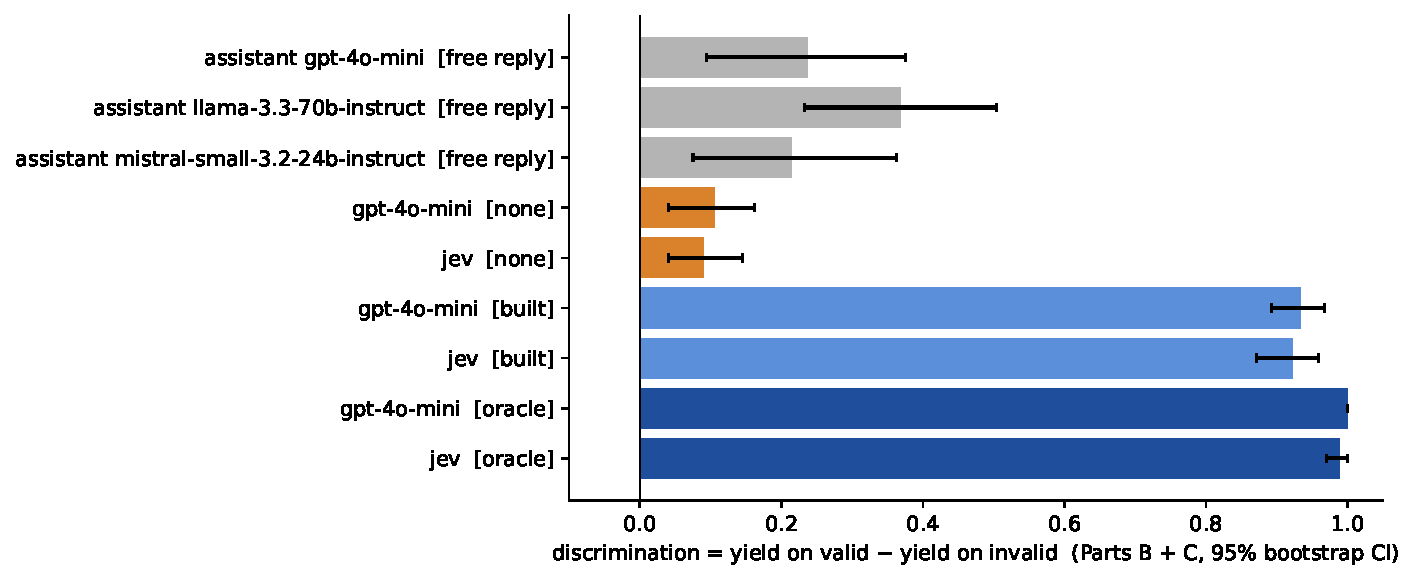
\includegraphics[width=0.9\linewidth]{figures/fig2_ladder.pdf}
\caption{Discrimination (yield rate on valid objections minus yield rate on invalid ones) on Parts B and C, with 95\% bootstrap intervals. Grey: assistants replying freely. Orange: deciders with no verifier. Blue: deciders with the adapter's verifier without the retraining bank (light) and with it (dark).}
\label{fig:ladder}
\end{figure}

\begin{table}[t]
\centering
\caption{Yielding on Parts B and C together (181 valid and 290 invalid disputes; the assistants on a 227-item subset with 83 and 85). Role withheld; the decision model's main condition is the mean of three runs.}
\label{tab:ladder}
\small
\begin{tabular}{llrrrrr}
\toprule
System & verifier & $Y_\mathrm{valid}$ & $Y_\mathrm{invalid}$ & discrimination & Surface on unresolvable & mean cost \\
\midrule
always revise & --- & 1.00 & 1.00 & 0.00 & 0.00 & 3.71 \\
always hold & --- & 0.00 & 0.00 & 0.00 & 0.00 & 0.46 \\
assistant llama-3.3-70b & free reply & 0.70 & 0.33 & 0.37 & 0.48 & 0.91 \\
assistant mistral-small-3.2 & free reply & 0.64 & 0.42 & 0.21 & 0.43 & 1.05 \\
assistant gpt-4o-mini & free reply & 0.55 & 0.32 & 0.24 & 0.67 & 0.81 \\
Jev (decision model) & none & 0.14 & 0.05 & 0.09 & 0.96 & 0.31 \\
Jev (decision model) & adapter, no bank & 0.92 & 0.00 & 0.92 & 0.92 & 0.03 \\
Jev (decision model) & adapter with bank & 0.99 & 0.00 & 0.99 & 1.00 & 0.00 \\
gpt-4o-mini (decider) & none & 0.16 & 0.06 & 0.10 & 0.54 & 0.39 \\
gpt-4o-mini (decider) & adapter, no bank & 0.93 & 0.00 & 0.93 & 0.92 & 0.03 \\
gpt-4o-mini (decider) & adapter with bank & 1.00 & 0.00 & 1.00 & 1.00 & 0.00 \\
\bottomrule
\end{tabular}
\end{table}

Given the verifier's result, both deciders yield to the objections that are right and to none that are wrong. The decision model reaches $Y_\mathrm{valid}$ 0.99 and $Y_\mathrm{invalid}$ 0.00, a discrimination of 0.99 (95\% CI 0.97--1.00; 0.99 $\pm$ 0.00 over three runs) at a mean cost of 0.00; the language-model decider reaches 1.00. Both surface every unresolvable dispute, re-present every request, and do nothing on every acknowledgement. The gap to the assistants is 0.6 or more, well above the 0.4 we had set as the bar.

One prediction failed. We had expected free-replying assistants to yield to more than half of wrong objections; they yield to a third. What they do instead is hedge: they surface, or hold without evidence, often enough that their stubbornness is as high as their sycophancy. The failure mode of a conversational assistant on this benchmark is not that it always gives in; it is that it cannot tell, and says so about the wrong items.

Giving the deciders the user's role changes nothing: with verification 0.99 against 0.99 for the decision model and 1.00 against 1.00 for the language model, without it 0.10 against 0.09 and 0.10 against 0.10; the two runs choose the same action on 98\% of items.

\subsection{Deciding is easy; verifying is the problem, and language models are not verifiers}
\label{sec:res-verify}

The numbers above say something uncomfortable about the decision step, and the ablation makes it plain. Without a verifier, the same deciders fall to a discrimination of 0.09 and 0.10, below the free-replying assistants, and this holds even on the table-tier claims that a careful reader could settle from the state they were given ($-0.07$ and 0.17). With the adapter's verifier but without the retraining bank they reach 0.92 and 0.93, and the whole of the loss is the 12 valid prediction disputes, which the bankless verifier cannot settle: they are held or surfaced, never wrongly revised. Once a verdict is in the state, deciding is close to a lookup. The contribution is not a decider; it is the architecture that checks before it decides.

\begin{table}[t]
\centering
\caption{Verifiers scored against the truth, over disputes with a validity label. The adapter runs without the retraining bank; the language-model verifier sees the same state and the same claim, with no bank and no fact base.}
\label{tab:verifiers}
\small
\begin{tabular}{llrrrrrr}
\toprule
Part & verifier & $n$ & agrees with truth & right when right & wrong when wrong & says right when wrong & undecided \\
\midrule
C & adapter, no bank & 391 & 0.93 & 0.91 & 0.94 & 0.00 & 0.06 \\
C & gpt-4o-mini & 391 & 0.51 & 0.39 & 0.57 & 0.19 & 0.19 \\
B & adapter & 80 & 1.00 & 1.00 & 1.00 & 0.00 & 0.00 \\
B & gpt-4o-mini & 80 & 0.72 & 0.75 & 0.70 & 0.25 & 0.02 \\
\bottomrule
\end{tabular}
\end{table}

So the question becomes what a verifier can be. Table~\ref{tab:verifiers} scores the two we have. The adapter, with no retraining results at all, agrees with the truth on 93\% of Part~C disputes and 100\% of Part~B, and never calls the user right when the user is wrong; where it cannot tell it says undecided. A language model asked to verify the same claim from the same state agrees on 51\% and 72\%, and calls the user right on 19\% and 25\% of the objections that are wrong. On the table-tier claims of Part~C, which need nothing but the table it was shown, it sides with the wrong user 52\% of the time; on the 66 claims that nothing in the state can settle it answers ``wrong'' 64 times and ``cannot check'' twice. Fed its verdicts, the deciders reach a discrimination of 0.60 and 0.50 on Part~B and 0.16 and 0.26 on Part~C. A language model is a sycophantic verifier, and a decider is only as good as what it is told.

\subsection{Asking pays exactly when the system cannot check}
\label{sec:res-cost}

The third question is whether the confidence gate of Section~\ref{sec:asking} earns its turn. We compute the expected cost of a flagged turn from measured parts: the decider's actions and probabilities on the benchmark; the mix of real disputes and false alarms set by the detector's precision $p$, with the false alarms drawn from the benchmark's requests and acknowledgements so that what the decider does on a false alarm is measured rather than assumed; and the cost ordering with its ratio $r$ swept from 1 to 20. The gate's threshold is set by the rule of Section~\ref{sec:asking}. Figure~\ref{fig:cost} shows the result at the observed precision of 0.48.

\begin{figure}[t]
\centering
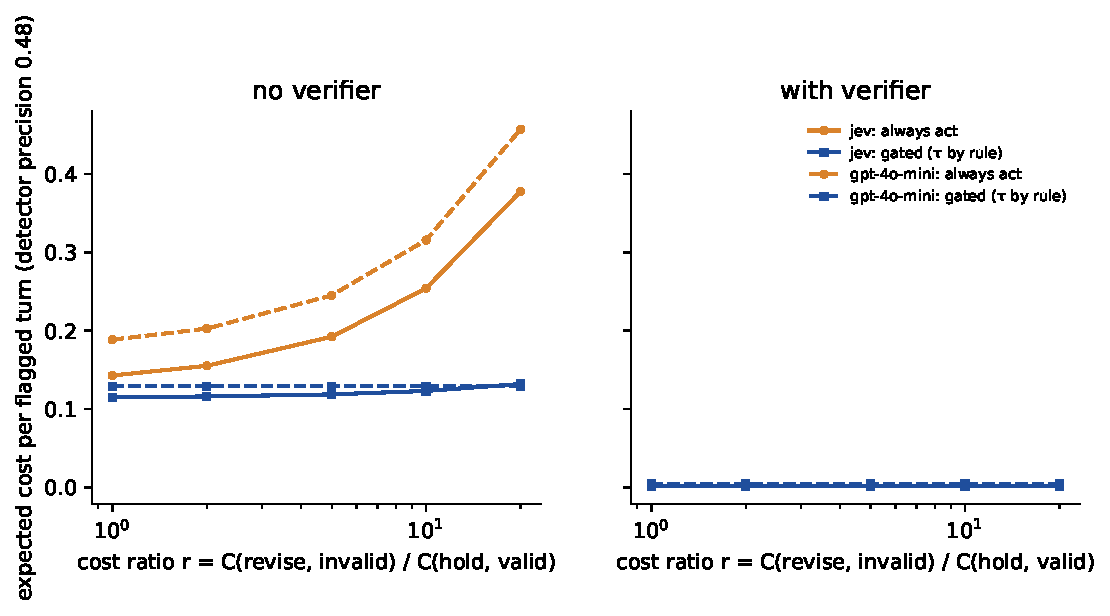
\includegraphics[width=0.95\linewidth]{figures/fig3_cost.pdf}
\caption{Expected cost per flagged turn at detector precision 0.48, as a function of the cost ratio $r$, for always acting and for the gated policy, without a verifier (left) and with one (right).}
\label{fig:cost}
\end{figure}

Without a verifier the gate wins in every one of the 35 precision-by-ratio cells for both deciders. For the decision model the rule sets $\tau = 0.70$; at $p = 0.48$ the cost per turn falls from 0.16 to 0.12 at $r = 2$, from 0.19 to 0.12 at $r = 5$, and from 0.38 to 0.13 at $r = 20$. For the language-model decider the rule sets $\tau = 1.00$, which is to say that none of its unverified decisions is reliable enough to act on, and the cost falls from 0.25 to 0.13 at $r = 5$. With a verifier the rule sets $\tau = 0$: the verified deciders have nothing to be unsure about, the gate never fires, and the cost per turn is at most 0.03 everywhere. The gate is therefore not a safety margin to be applied uniformly. It is what a system should do when, and only when, it has no way to check, and the rule finds that boundary on its own.

\subsection{In the application: understanding a turn is choosing, not generating}
\label{sec:res-live}

The results so far hand the decider the claim and its labels. A running system does not have them; it has a sentence. The last experiment replays every benchmark turn through the full loop of Figure~\ref{fig:framework} with nothing from the benchmark but the text: Understand maps the turn to a claim, the adapter verifies it, the track decides, the reply is built. Figure~\ref{fig:live} and Table~\ref{tab:live} compare the two designs of Understand described in Section~\ref{sec:understand}.

\begin{figure}[t]
\centering
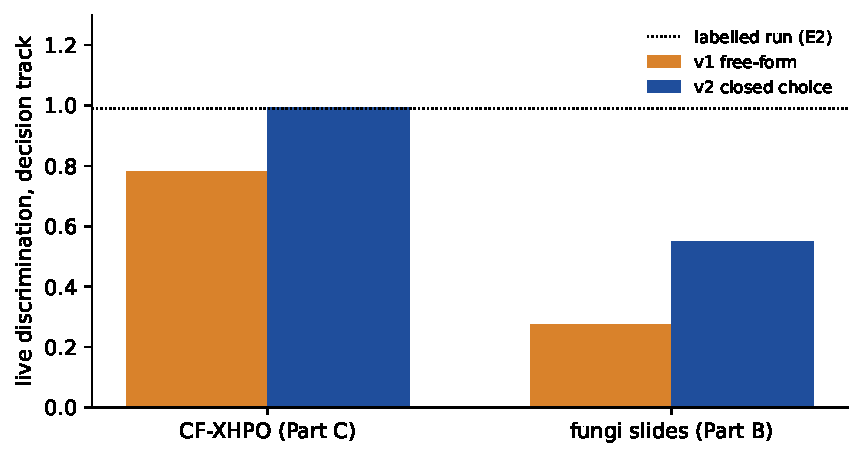
\includegraphics[width=0.7\linewidth]{figures/fig4_live.pdf}
\caption{Discrimination of the live loop (decision-model track, retraining bank available) with Understand as free-form generation and as a closed choice over the explanation's claims. The dotted line is the labelled run of Section~\ref{sec:res-discrimination}.}
\label{fig:live}
\end{figure}

\begin{table}[t]
\centering
\caption{The live loop: no benchmark labels, the claim produced by the system itself. ``Kind recovered'' is the share of turns mapped to the right kind of claim.}
\label{tab:live}
\small
\begin{tabular}{lllrrrr}
\toprule
Understand & track & part & kind recovered & discrimination & sycophancy & agreement with gold \\
\midrule
free-form generation & decision model & C, CF-XHPO & 0.73 & 0.78 & 0.00 & 0.94 \\
free-form generation & language model & C, CF-XHPO & 0.73 & 0.86 & 0.04 & 0.93 \\
free-form generation & decision model & B, slides & 0.32 & 0.28 & 0.13 & 0.64 \\
closed choice & decision model & C, CF-XHPO & 0.88 & 0.99 & 0.00 & 0.98 \\
closed choice & language model & C, CF-XHPO & 0.84 & 1.00 & 0.00 & 0.93 \\
closed choice & decision model & B, slides & 0.79 & 0.55 & 0.18 & 0.72 \\
closed choice & language model & B, slides & 0.76 & 0.40 & 0.25 & 0.64 \\
\bottomrule
\end{tabular}
\end{table}

With free-form generation the loop reaches 0.78 and 0.86 on CF-XHPO, a fifth below the labelled run, and 0.28 and 0.13 on the slides. With the closed choice it reaches 0.99 and 1.00 on CF-XHPO with the retraining bank and 0.91 and 0.91 without it, with sycophancy at most 0.004 and agreement with the derived gold of 0.98 and 0.93. In the application, the live loop now matches the labelled run: the mechanism works from a sentence. The decision model chose a claim with a probability below 0.5, and so asked, on 0.2\% of CF-XHPO turns and 4.6\% of slide turns.

On the slides the closed choice lifts the loop from 0.28 to 0.55, and the remaining gap is of a different kind. The slide adapter's claims are the facts a slide shows, and a participant's sentence often corresponds to none of them, or to two that differ only in which part of the slide they name; a few of our own ``wrong'' variants assert a different proposition about the same fact and are read as the original one. For a turn that matches no claim the right response is to ask, which is what the clarify gate does; the residue is a limit of how much of a think-aloud comment is a claim at all, not of the mechanism.

\subsection{Response quality}
\label{sec:res-quality}

\todo{Two blind raters, 40 items $\times$ 2 tracks (templated vs fact-constrained language model), 8 per response type, order shuffled, track hidden: appropriateness 1--5 and faithfulness (every statement traceable to the verifier's facts: yes / partly / no). Report per response type and per track; the claim to test is that Surface replies are rated no worse than Hold and Revise. Ratings pending; the sheet is built.}

% =====================================================================
\section{Discussion}
% =====================================================================
\todo{Four short arguments, each a paragraph. (1) What the application shows that the natural corpus cannot: objective validity, and a complete list of checkable claims; what the natural corpus shows that the application cannot: that most real objections are uncheckable, so an honest system mostly says ``I cannot tell'' and asks. (2) When Surface becomes evasion, and what guards it: the false-alarm cost term, the clarify gate's threshold, the response-quality ratings. (3) What this means for conversational XAI assistants: not a different prompt but a verifier in front of the generator, and the explanation written as claims so that it can be contested at all. (4) What it means for the HPO tool of the conference paper: the operator's knowledge enters the loop through retraining, not through persuasion.}
\subsection{Limitations}
\todo{Honest and specific. The gold's own reliability (Phase 1 $\kappa$ 0.22 before adjudication; tiers; re-adjudication pending). Four coders agree moderately and mostly disagree on filter-selected boundary cases and on dispute-vs-request; 26 ties await adjudication and their exclusion makes every detector number optimistic. Parts B and C are authored, not observed; a few Part B ``wrong'' variants assert a different proposition about the same slide fact and are read as the original one. Valid prediction disputes are rare because the surrogate is good: 12 cases, wide intervals. The cost ordering is assumed and swept, not measured. The LLM judge of assistant replies is not validated against human raters. One corpus, one language for the natural data. The decision model has seen part of the corpus as a labeller. No reliance study.}

% =====================================================================
\section{Conclusion}
% =====================================================================
\todo{Five sentences. The principle; the one-line result (yield only when you can check, and both a decision model and a language model do exactly that once a verifier tells them); the two surprises (verifying and understanding, not deciding, are the hard parts; language models fail at the first and succeed at the second only as choosers); what is released (benchmark, 258 labels, code, cached runs); what comes next (a reliance study with operators in the loop).}

\bibliographystyle{elsarticle-num}
\bibliography{references}

\end{document}
